
\newcommand{\PaperTitleSize}{Clusters in intense XUV pulses: Effects of cluster size on expansion
                             dynamics and ionization}

\publication{\PaperTitleSize}
\label{section:papers:size}

\begin{flushright}
Edward Ackad, Nicolas Bigaouette, Kyle Briggs and Lora Ramunno\\
\textit{Physical Review A} 83(6), June 2011, 063201\\
\href{http://dx.doi.org/10.1103/PhysRevA.83.063201}{doi:10.1103/PhysRevA.83.063201}
\end{flushright}


% Include PDF's abstract in the Table-of-Content as ``subsection 0'' but hide the number
\HidePDFAbstractNumber

\subsection{Author contributions}
The MD package was mostly written by N. B. Most post processing scripts used to
analyze data and generate figures were written by N. B. and tweaked by E. A.
The article text was written by E. A. with some corrections by N. B. Data
acquisition was done by both N. B. and E. A. All authors contributed to the
discussion.


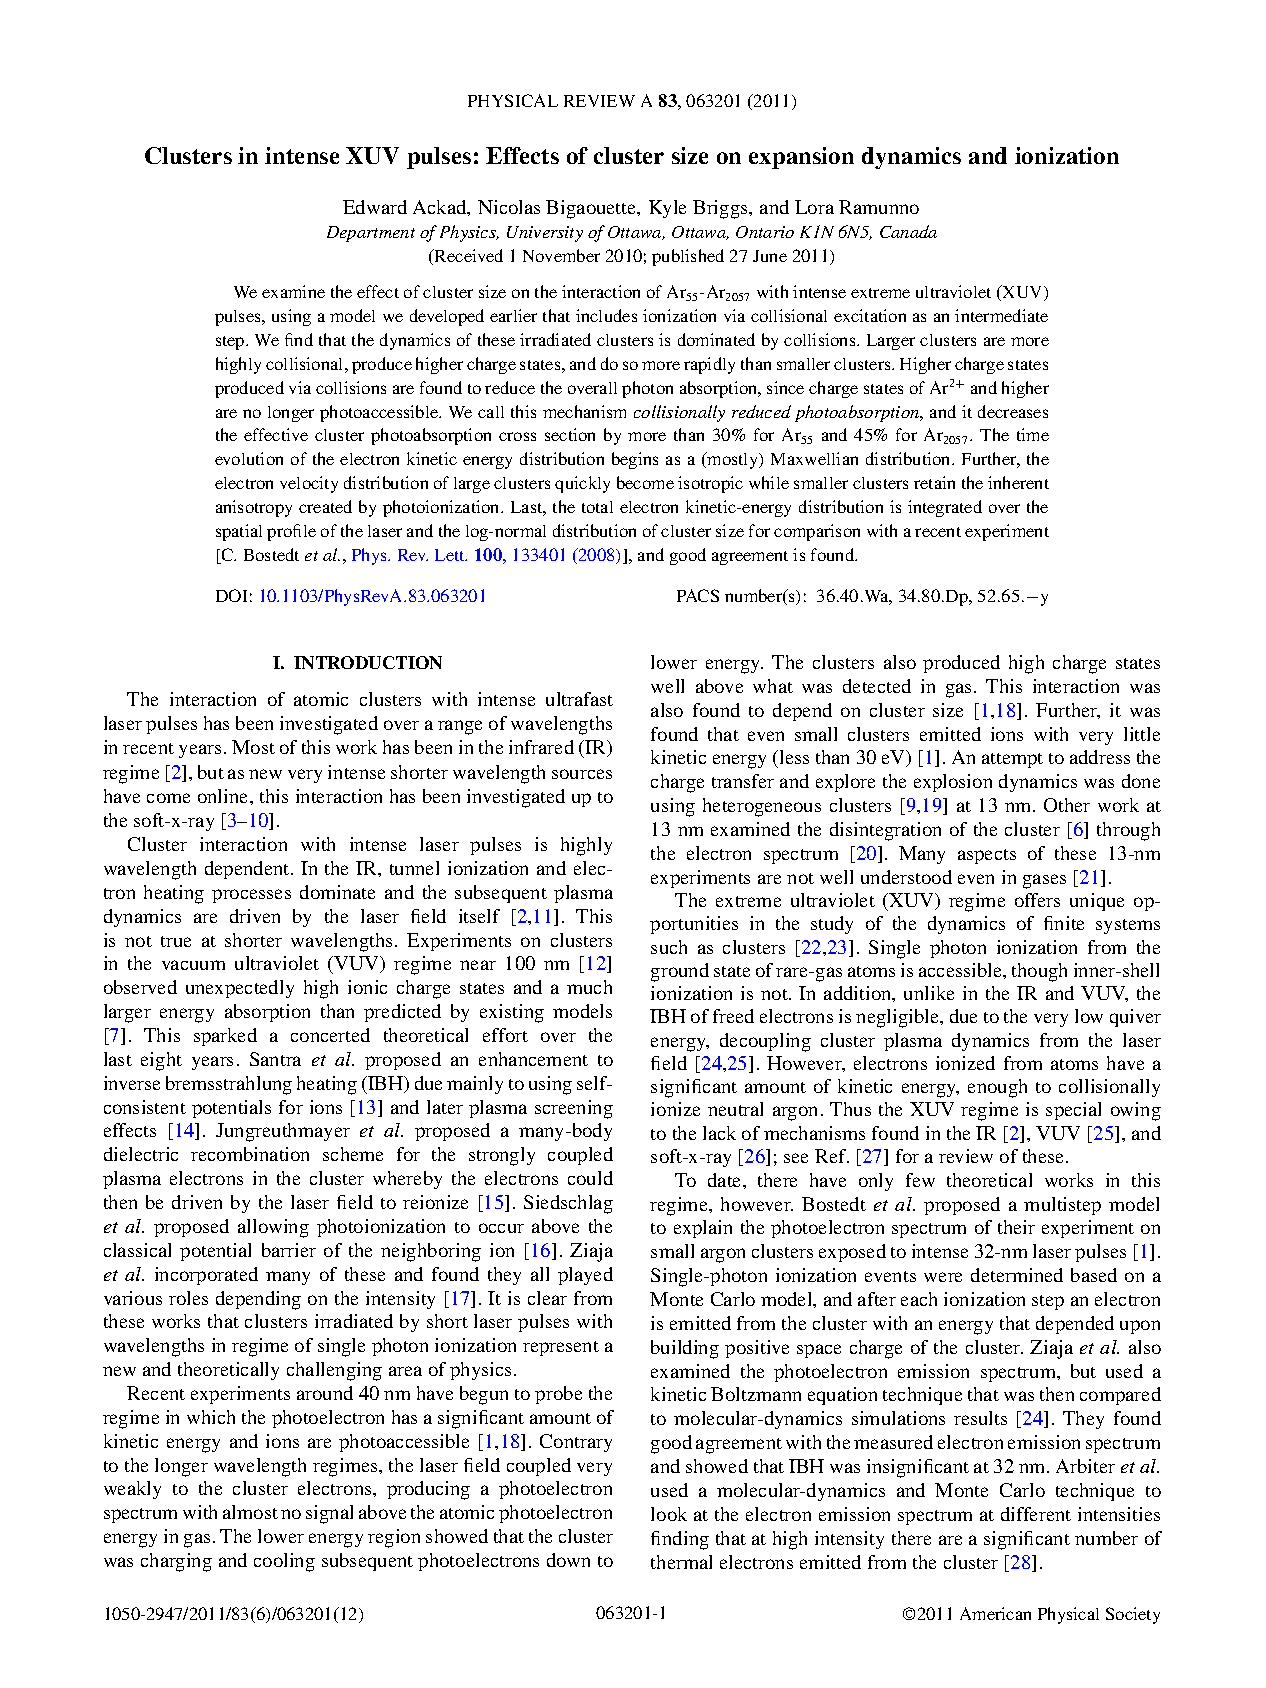
\includepdf[pages=-,
            addtotoc={
                %1,section,1,{\PaperTitleSize},paper_size,
                1,subsection,2,Abstract,paper_size_abstract,
                1,subsection,2,Introduction,paper_size_intro,
                2,subsection,2,Theory,paper_size_theory,
                3,subsection,2,Results,paper_size_results,
                3,subsubsection,3,Ions,paper_size_ions,
                3,paragraph,4,Charge state,paper_size_cs,
                3,paragraph,4,Charge state evolution,paper_size_cs_ev,
                5,paragraph,4,Excited states evolution,paper_size_es_ev,
                5,paragraph,4,Mechanisms of ionization,paper_size_ionization,
                6,paragraph,4,Charged shell structure,paper_size_shell,
                7,paragraph,4,Kinetic energy,paper_size_K,
                8,subsubsection,3,Electrons,paper_size_electrons,
                8,paragraph,4,Kinetic energy distribution,paper_size_distrib_K,
                9,paragraph,4,Velocity distribution,paper_size_distrib_v,
                10,paragraph,4,Connection with experiment,paper_size_exp,
                10,subsection,2,Summary,paper_size_summary,
                11,subsection,2,Acknowledgements,paper_size_ack,
                11,subsection,2,References,paper_size_ref
            }]{papers/Ackad2011b.pdf}
